\chapter{Feed-Forward neural networks}
To understand the technique used in this report, it is necessary to understand basic neural networks functioning.
Given a scenario with a training set of labeled data $(\textbf{x}, \textbf{y})$, where $\textbf{x}$ denotes the training example
composed of multiple features, say $\textbf{x} = \{x_{1}, x_{2}, \ldots, x_{n}\}$, and \textbf{y} the corresponding label.
Let's introduce the idea of `perceptron'. \\
Perceptrons are the building blocks of neural networks, and the best way to get stated is with an example.
Assume at the university's admission office the students are evaluated with two pieces of information, the results of a test and their grades in school. Let's take a look at some sample students, see \cref{fig:perceptron}.

\begin{figure}[ht]
  \centering
  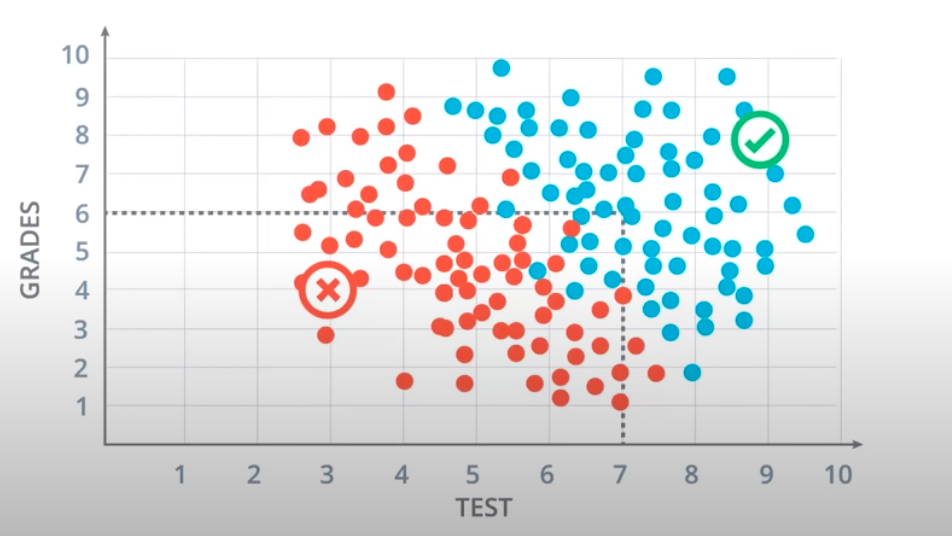
\includegraphics[width=0.7\textwidth]{figs/fig1.png}
  \caption{test vs grades }\label{fig:perceptron}
\end{figure}

The data on the figure can be nicely separated with a line, where most students above the line get accepted and most students under the line get rejected, see \cref{fig:line}. Therefore this line is going to be our model. \\
The model makes a couple of mistakes since there are a few blue points that are under the line and few over the line, but they are considered as noise and add no new information to our model. Now, the natural question that arises: how do we find the line ?

\begin{figure}[htbp]
  \centering
  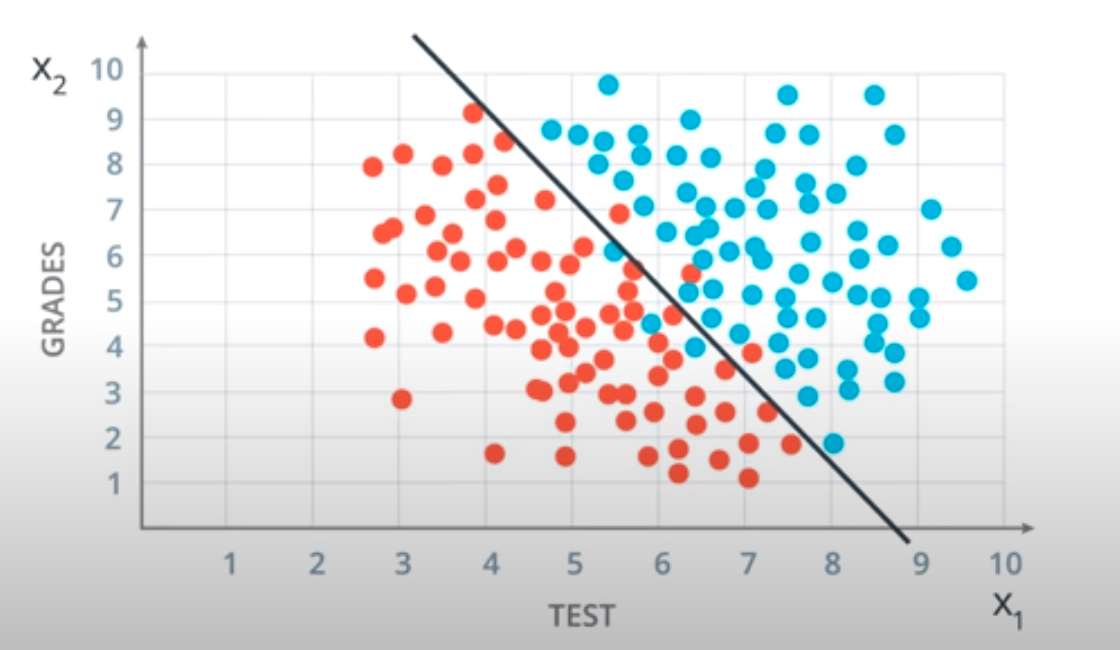
\includegraphics[width=0.7\textwidth]{figs/fig2.png}
  \caption{seperating line}\label{fig:line}
\end{figure}

We start by labeling the axis $\textbf{x} = \{x_{1}, x_{2}\}$.
The boundary line separating the students has a linear equation
specifically: $2x_{1} + x_{2} - 18 = 0$.
Plotting the grades in the equation gives rise to a score, if the score is positive --the student
gets plotted in above the line--, the student gets accepted with otherwise not. This is called a prediction.\\

In a more general case, our boundary will be an equation of the following form:

$$w_{1}x_{1} + w_{2}x_{2} + b = 0.$$

Abbreviating this equation into vector notation:

\begin{equation}
  \label{linear}
  \textbf{w}\cdot\textbf{x} + b = 0
\end{equation}

Where $\textbf{w} = \{w_{1}, w_{2}\}$. We refer to $\textbf{x}$ as the input, $\textbf{w}$ as the weights and $b$ as the bias. Here $\textbf{y} = \{0, 1\}$ is the label, where 0 indicates the student being rejected whereas 1 indicates the student being accepted. Finally, our prediction is going to be called \mbox{\boldmath{$\hat{y}$}} and it will be what the algorithm predicts that the label will be, namely:

\begin{equation}
  \label{y_hat}
  \hat{y} =
  \begin{dcases*}
    \text{1,}  &$w\cdot x + b \geq 0$ \\
    \text{0,}  &$w\cdot x + b < 0$
  \end{dcases*}
\end{equation}

and the goal of the algorithm is to have \mbox{\boldmath{$\hat{y}$}} resembling \mbox{\boldmath{$y$}} as closely as possible. Reorganizing the equations in a graph and generalizing, gives rise to \cref{fig:neuron}. Here the bias is consider as a dummy input with value 1 to the Perceptron with weight b.

% \afterpage{\cleardoublepage}
\begin{figure}[H]
  \centering
  \includegraphics[width=0.7\textwidth]{figs/perceptron.png}
  \caption{perceptron's graph representation}\label{fig:neuron}
\end{figure}

% \section{activation functions}
%
% Giving a training set, the classification of the input vector is based upon $\textbf{w}$, therefore the goal of the algorithm is to determine those
% weights through an iterative process. The probelm given here is that the algorithm can only learn linear functions since the output of the perceptron
% is a simple linear combination of the input. In real world situation, the data is much more complex and highly non-linear, therefore to remedy this
% problem we shall introduce a non-linearty in our algorithm, called \textbf{activation function} in deep learning literature. Namely the sigmoid
% function.
%
% $$
% \sigma(x) = \frac{1}{1 + e^{-x}}
% $$
%
% One important property of an activation function is differentiability, because as we are going to explore in section, gradient descent will be used as optimizer to determine the networks' weights, in contrast to the perceptron which uses a discrete activation. That sigmoid function can be seen as continuous version of the perceptron's discrete activation function. Indeed:
%
%
%
%
% Instead of returning 0 or 1, the sigmoid function returns the probability of an event occuring, thus in our example the sigmoid function would output
% the probability of a student getting accepted or rejected, which can be expressed as the the conditional probability $p(y=1 | x) = \sigma(w\cdot x +
% b)$. There several other activation functions that can be used depending on the problem at hand. For example if a neural network is used to predict
% continuous non-bounded function that takes values in the interval $]-\infty, +\infty[$, then a more clever choice is the linear activation
% funciton, which is defined as: $f(x) = x$.


\section{Cost function}\label{cost}

In order to estimate the accuracy of the algorithm, or otherwise stated determine how well a certain prediction given by the algorithm is, we may establish a cost function, which measures the error the algorithm makes on some prediction (cost function is often referred to as error function). There are more that one choice for such a function. \Cref{equ:mse} can be used, it is called ``The Mean Squared Error''.

\begin{equation}
  \label{equ:mse}
  L(w, b) = \frac{1}{2} \sum_{i = 1}^{n} ||y - \hat{y}||^2.
\end{equation}

This function, becomes large when our network approximates $y$ badly, and small when the approximation is accurate. Additionally notice that if we set $L_x = \frac{1}{2} (y - \hat{y})^2$ we have that:
\begin{equation}
  \label{equ:additivity}
  L(w,b) = \sum_{i = 1}^{n} L_{x_{i}}.
\end{equation}
This property will be important in the algorithm described in Section 2.2.3.

Another way of defining a cost function is using the ``The Maximum Likelihood Estimation'' technique, since the sigmoid function deals with probabilities. We take the joint probability of the entire training set, assuming the training examples being independent events:

\begin{equation}
  \label{equ:likelihood}
  L(w, b) = p(y^{(1)}, y^{(2)}, \ldots, y^{(n)} | x^{(1)}, \ldots, x^{(n)}) = \prod_{i=1}^{n} p(y^{(i)}|x^{(i)})
\end{equation}

where $x^{(i)}$, $y^{(i)}$ represent the $i^{th}$ training example and label respectively. Thus by maximizing the joint probability, or respectively minimizing the $-\log$ of the likelihood, we can get an estimate of the parameters $w \ and \ b $. Now, in our worked example, the neural network can be treated as a random variable having a Bernoulli distribution, therefore \cref{equ:likelihood} can be rewritten as follows:

\begin{equation}
  \label{equ:b_likelihood}
  L(w, b) = - \sum_{i = 1}^{n} y_i \log(\hat{y}) + (1 - y) \log(1 - \hat{y}).
\end{equation}

\Cref{equ:b_likelihood} is usually the cost function used for Bernoulli distributed labeled data. It is often referred to as \textbf{binary cross-entropy} or BCE for short.

For multi-class classification (predicting multiple classes, say $k$ classes), a similar idea can used considering a multinoulli distribution on the data set where $p(y | \textbf{x}) = \prod_{i = 1}^{k} p_i^{[y=i]}$, where $[y = i]$ evaluates to 1 if $x = i$, 0 otherwise. This leads to following cost function using MLE

\begin{equation}
  \label{equ:m_likelihood}
  L(w, b) = - \sum_{j = 1}^k \sum_{i = 1}^{n} y_{i, j} \log(\hat{y}_{i, j}).
\end{equation}

\section{Gradient descent}
In order to minimize the cost function we rely on optimization algorithms from numerical methods as it is unpractical to solve manually. The technique used in deep learning is the gradient descent. \\
The gradient of a differentiable function $f: \mathbb{R}^n \longrightarrow \mathbb{R}$ at a point $x = (x_1, \ldots, x_n) \in \mathbb{R}^n$ is a vector in $\mathbb{R}^n$ of the form

\begin{equation}
  \label{equ:gradient}
  \nabla f(x) = (\frac{\partial f}{\partial x_1} (x), \ldots, \frac{\partial f}{\partial x_n} (x))
\end{equation}

It is a well known result that, given a point $x \in \mathbb{R}^n$, the gradient at that point the direction of steepest ascent. Given that $f$ is differentiable at $x$, the vector $-\nabla f(x)$ indicates the direction of steepest descent of the function $f$ at the point $x$.
In order to obtain the minimum value of the function, the gradient descent strategy tells us to start at a given $x_0 \in \mathbb{R}^n$, calculate the value of $\nabla f(x_0)$, and then proceed to calculate a new point $x_1 = x_0 − \alpha \nabla f(x_0)$, where $\alpha > 0$ is called the \textbf{learning rate}. We then repeat this process, creating a sequence $\{ x_i \}$ defined by our initial choice of $x_0$, the learning rate $\alpha$, and the rule: $x_{i + 1} = x_{i} − \alpha \nabla f(x_0)$  . This sequence continues until we approach a region close to our desired minimum.
The method of gradient descent when taken continuously over infinitesimally small increments (that is, taking the limit $\alpha \rightarrow 0$) usually converges to a local minimum. However, depending on the location of the initial $x_0$, the local minimum achieved may not be the global minimum of the function. Furthermore, since when carrying out calculations on an unknown function we must take discrete steps (which vary in length depending on the learning rate), we are not even guaranteed a local minimum but rather may oscillate close to one, or even ’jump’ past it altogether if the learning rate is too big. Still, even with these possible complications, gradient descent is a surprisingly successful method for many real life applications and is the most standard method of training for feed-forward neural networks and many other machine learning algorithms.
Given that our cost function indicates how poorly our neural network approximates a given function, by calculating the gradient of the cost function with respect to the weights and biases of the network and adjusting these parameters in the direction opposite to the gradient, we will decrease our error and therefore lead us closer to an adequate network (in most cases) see .

\subsection{Gradient calculation}\label{sec:cal_gradient}

Before applying the gradient descent technique, we can clearly see that the an output of 0 or 1 is problematic since the derivatives would be 0. Therefore the gradient descent technique will not work. To remedy this, following the MLE, a Bernoulli distribution has been defined on $y$, therefore the neural net needs to predict $\yhat = p(y = 1 | x) = \sigma (x)$. For this number to be a valid probability, it must lie in the interval $[0, 1]$. \\
A good approach would ensure the existence of a strong gradient whenever the model has the wrong answer. And for consistency with the perceptron's decision rule (\cref{y_hat}), a very positive linear combination of the input $x$ has to have a probability close to 1 and vise versa (see \cref{fig:step_sigmoid}), otherwise

\begin{equation}
  \label{equ:limits}
  \lim_{x \rightarrow +\infty} \sigma(x) = 1, \qquad \lim_{x \rightarrow -\infty} \sigma(x) = 0.
\end{equation}

This approach is based on the sigmoid function:
 $$
 \sigma(x) = \frac{1}{1 + e^{-x}}
 $$

This function is suitable for the problem at hand, namely binary classification. However, depending on the output $\yhat$ other functions might be used. For example if a neural network is used to predict continuous non-bounded function that takes values in the interval $]-\infty, +\infty[$, then a more clever choice is the linear activation function, which is defined as: $f(x) = x$. Another example is the multi-class classification, where a multinoulli distribution is defined over the training data. The function used is the softmax defined as

$$
softmax(x_i) = \frac{e^{x_i}}{\sum_j e^{x_j}}
$$

Where $x_i$ represents a training example from class $i$. Here the output consists of $j$ outputs rather that a single one. See \cref{fig:ann} to illustrate the output layer.

\begin{figure}[!htpb]
  \centering
  \includegraphics[width=\textwidth]{figs/step_sigmoid.png}
  \caption[sigmoid vs step function]{sigmoid vs step function. The two plots clearly show cast the continuity of the sigmoid.}\label{fig:step_sigmoid}
\end{figure}

Now, let us apply the gradient descent technique to our network. Our goal is to calculate the gradient of $L$ at a point $x = (x_1, \ldots, x_n)$ given by the partial derivatives, see \cref{equ:gradient}. In addition, the property \cref{equ:additivity} now become important. In fact, we are only going to calculate the value of $\nabla L_x$ for a given labeled data point and then add the values of the gradient together, see below.

\begin{equation}
  \nabla L(w, b) = \nabla (\sum_{i = 1}^{n} L_x) = \sum_{i = 1}^{n} \nabla L_{x_i}.
\end{equation}

The error produced by each point is simply: $ L_x = -y \log (\hat{y}) - (1 - y) \log (1 - \hat{y})$. In order to calculate the derivative of this error with respect to the weights, we'll first calculate $ \frac{\partial}{\partial w_j} \hat{y}$, where $ \hat{y} = \sigma (w \cdot x + b)$.

\begin{align*}
  \frac{\partial}{\partial w_j} \hat{y} &= \frac{\partial}{\partial w_j} \sigma (w \cdot x + b) \\
     &= \sigma (w \cdot x + b) (1 - \sigma (w \cdot x + b)) \cdot \frac{\partial}{\partial w_j} (w \cdot x + b) \\
     &= \hat{y} (1 - \hat{y}) \cdot \frac{\partial}{\partial w_j} (w \cdot x + b) \\
     &= \hat{y} (1 - \hat{y}) \cdot \frac{\partial}{\partial w_j} (w_1 x_1 + \ldots + w_j x_j + \ldots w_n x_n + b) \\
     &= \hat{y} (1 - \hat{y}) \cdot x_j.
\end{align*}

Now we can go ahead and calculate the derivative of the error $L$ at a point $x$, with respect to the weight $w_j$.

\begin{align*}
  \frac{\partial}{\partial w_j} L_x &= \frac{\partial}{\partial w_j} [-y \log (\hat{y}) - (1 - y) \log (1 - \hat{y})] \\
     &= -y \frac{\partial}{\partial w_j} \log (\yhat) - (1 - y) \frac{\partial}{\partial w_j} (1 - \yhat) \\
     &= -y \frac{1}{\yhat} \cdot \frac{\partial}{\partial w_j} \yhat - (1 - y) \frac{1}{1 - \yhat} \cdot \frac{\partial}{\partial w_j} (1 - \yhat) \\
     &= -y (1 - \yhat) \cdot x_j + (1 - y)\yhat \cdot x_j \\
     &= -(y - \yhat) x_j
\end{align*}

A similar calculation will show that

$$
\frac{\partial}{\partial b} L_x = -(y - \yhat)
$$

Therefore, since the gradient descent step simply consists in subtracting a multiple of the gradient of the error function at every point, then this updates the weights in the following way:

\begin{align}
  w^{\prime}_i &= w_i + \alpha (y - \yhat)x_i \\
  b^{\prime} &= b + \alpha (y - \yhat)
\end{align}

\section{Neural network architecture}
In our work example, the target function was a simple linear function. However, in real world situations the input data is much more complex and often cannot be separated with a line. That is where neural nets shine. Neural networks also referred to as \textbf{feedforward} neural nets or \textbf{multilayer perceptron} (MLPs) are as the name indicates are stacks of perceptrons, where each \textbf{unit} receives the input $x$, calculates the inner product with a set of weights and apply a non-linearity to the result, then these results are fed to a next layer of units that does the same calculations and so on. The overall length of the chain gives the \textbf{depth} of the model. The final layer of such a network is called the \textbf{the output layer}, whereas the intermediate layer are referred to as \textbf{hidden layers}. The goal of the feed-forward network is to approximate some function $f^*$. The training example specify directly what the output layer must do at each point $x$; it must produce a value that is close to $y$. Therefore, the function computed after the linear combination is important. This function and the functions used in the hidden layers are referred to as \textbf{activation functions}. For example for a classifier, the function maps an input $x$ to a category $y$, a natural choice of activation is the sigmoid; whereas in a regression problem, where the output is continuous non-bounded that takes values in the interval $]-\infty, +\infty[$, a more clever choice is the linear activation function, which is defined as: $f(x) = x$.
The figure below depicts the architecture described above.

\begin{figure}[!htpb]
  \centering
  \includegraphics[width=\textwidth]{figs/nn.png}
  \caption[A visual representation of a feed-forward network]{A visual representation of a feed-forward network which approximates some function $f : \mathbb{R}^n \longrightarrow \mathbb{R}^m$ by
    computing the function $f^*(x) = (f^*_1(x), \ldots, f^*_m(x))$. In this approach, the network is shown as a
    directed weighted graph. Here $x = (x_1, \ldots, x_n)$}\label{fig:ann}
\end{figure}

For notation, set $w^n_{a, b} \in \mathbb{R}$ as the weight between the $a^th$ unit in the $(n - 1)^th$ layer with $k$ units to the $b^th$ unit in the $n^th$ layer with $j$ units.

\begin{equation}
  w_n = \begin{pmatrix}
    w^n_{1, 1} & \ldots & w^n_{1, k} \\
    \vdots & \ddots & \vdots \\
    w^n_{j, 1} & \ldots & w^n_{j, k}
  \end{pmatrix}
\end{equation}

The bias can be added as a dummy unit with input $x_{n+1} = 1$, which is a constant $b \in \mathbb{R}^j$. In order to calculate the output $a_n$ of the $n^th$ layer, we use the formula

$$
a_n = \sigma (w_n \cdot a_{n - 1} + b_n).
$$

In the above equation, the activation function $\sigma$ is applied element-wise to each element of the resulting vector. As the computations are carried out along the network's layers, the final function $f$ calculated by a network of depth $N$ is

$$
f(x) = \sigma(w_N\sigma(\ldots\sigma (w_2 \sigma(w_1 \cdot x + b_1) + b_2)) + b_N)
$$

\section{Back-propagation}
In order to train a neural network, the same techniques are used as in \cref{sec:cal_gradient}. First we define a cost function (which is the same as in the perceptron algorithm \cref{equ:b_likelihood},but with a much more complex $\yhat$), we calculate the feed-forward pass (we calculate the output $\yhat$), and then calculate the the gradient of the cost function $L$ with respect to every single weight and bias in the network, we get the following gradient vector $\nabla L = (\ldots, \frac{\partial}{\partial w^l_{i, j}} L, \ldots)$. Then applying the gradient step look likes

\begin{align*}
  w^{\prime l}_{i, j} &= w^l_{i, j} - \alpha  \frac{\partial}{\partial w^l_{i, j}} L\\
  b^{\prime l}_j &= b_j - \alpha \frac{\partial}{\partial b^l_j} L
\end{align*}

The big challenge of applying gradient descent to neural networks is calculating these partial derivatives.  This is where back-propagation comes in. This algorithm first tells us how to calculate these values for the last layer of connections, and with these results then inductively goes "backwards" through the network, calculating the partial derivatives of each layer until it reaches the first layer of the network. Hence the name "back-propagation".

For the purpose of this section it is useful to consider the values of each layer before the activation function step. Consider

\begin{equation*}
  z^l_j = \sum_k w^l_{j, k} a^{l - 1}_k + b^l_j \qquad \text{so that} \qquad a^l_j = \sigma (z^l_j).
\end{equation*}

Additionally, we denote the following:

\begin{equation}
  \delta^l_j = \frac{\partial}{\partial z^l_j} L
\end{equation}

This value will be useful for propagating the algorithm backwards through the network and directly related to $\frac{\partial}{\partial w^l_{i, j}} L$ and $\frac{\partial}{\partial b^l_j} L$ by the chain rule. since

\begin{align}
  \frac{\partial L}{\partial w^l_{i, j}}  &= \frac{\partial L}{\partial z^l_j} \frac{\partial z^l_j}{\partial w^l_{i, j}} = \delta^l_j a^{l - 1}_i \\
  \frac{\partial L}{\partial b^l_j} &= \frac{\partial L}{\partial z^l_j} \frac{\partial z^l_j}{\partial b^l_j} = \delta^l_j.
\end{align}

The value $a^{l - 1}_j$ has already been calculated through the forward pass. The only remaining term to calculate is $\delta^l_j$ and we obtain our gradient. Our first step is calculating this value for the last layer of the network, that is, $\delta^N_j$ for a network with $N$ layers. Since $a^{N}_j = \sigma (z^N_j)$, again using the chain rule

\begin{equation}
  \delta^N_j = \frac{\partial L}{\partial a^N_j} \frac{\partial a^N_j}{\partial z^N_j} = \frac{\partial L}{\partial a^N_j} \sigma^{\prime}(z^N_j)
\end{equation}

which can be easily calculated by a computer if we know how to calculate $\sigma^{\prime}$ (which should be true for any practical activation function).

Now we will only need to "propagate" this backwards in the network in order to obtain $\delta^{N - 1}_j$. In order to do so, apply the chain rule once again

\begin{align*}
  \delta^{N - 1}_j &= \frac{\partial L}{\partial z^{N - 1}_j} \\
                   &= \sum_i^k \frac{\partial L}{\partial z^{N}_i} \frac{\partial z^N_i}{\partial z^{N - 1}_j} \\
                   &= \sum_i^k \delta^N_i \frac{\partial z^N_i}{\partial z^{N - 1}_j}.
\end{align*}

If we focus on the term $\frac{\partial z^N_i}{\partial z^{N - 1}_j}$, we find that
\begin{align*}
  \frac{\partial z^N_i}{\partial z^{N - 1}_j} & = \frac{\partial (\sum_k w^N_{i, k} a^{N - 1}_k + b^N_i)}{\partial z^{N - 1}_j} \\
                &= \frac{\partial (w^N_{i, j} \sigma (z^{N - 1}_j))}{\partial z^{N - 1}_j} \\
                &= w^N_{i, j} \sigma^{\prime} (z^{N - 1}_j)
\end{align*}

which, again, can be easily calculated by a computer given the network. Therefore

\begin{equation}
  \delta^{N - 1}_j = \sum_i^k \delta^L_i w^N_{i, j} \sigma^{\prime} (z^{N - 1}_j).
\end{equation}

This formula tells us how to calculate any $\delta^l_j$ in the network, assuming we know $\delta^{l+1}$. We finally developed a way to
calculate all the $\delta^l_j$ ’s, given that we know what the values of $\delta^{l + 1}_j$  are. Thus, by propagating this method backwards through the layers of the network we are able to find all our desired partial derivatives, and can therefore calculate the value of $\nabla L$ as a function of the weights and biases of the network and execute the method of gradient descent.

\section{Problems related to neural nets}

Neural networks are extremely powerful function approximators, but during the design of architecture care should be taken since there are many parameter one can tune (depth, number of units in each layer, \ldots). Therefore, a complex design namely high number of units in each layer and a deep network can lead to \textbf{overfitting}. Over-fitting is the case where the overall cost is really small (The network is doing very well on the training set) but the generalization of the model to unseen data is poor and unreliable. There are many solutions proposed to break this effect such as \emph{dropout} which consists of randomly zeroing the output of some units in each layer to force the algorithm to take different routes through the network. This has the effect of training smaller portions of the network, and thus smaller functions with reduced complexity are learned. This has the effect of reducing the high variance of the overall neural net. This is referred to as \textbf{regularization}. \\
Another famous problem neural nets suffer from is \textbf{local minimum} problem, The error surface of a complex network is full of hills and valleys. Because of the gradient descent, the network can get trapped in a local minimum when there is a much deeper minimum nearby. A suggested solution is to increase the number of hidden units. This technique works because of the higher dimensionality of the error space, making the chance to get trapped smaller \cite{atnn}. \\
Another issue in deep neural nets is the \textbf{vanishing gradients} problem. As we learned from backp-ropagation, each of the neural network's weights receive an update proportional to the partial derivative of the error function with respect to the current weight in each training iteration. The problem is that in some cases, the gradient will be vanishingly small, eventually preventing the weight from changing its value. In the worst case, this may completely stop the neural network from further training. As the network trains, the weights can be adjusted to very large values. The total input of a hidden unit or output unit can therefore reach very high (either positive or
negative) values, and because of the sigmoid activation function the unit will have an activation very close to zero or very close to one \cite{atnn}. And since back-propagation computes gradients using the chain rule, this has the effect of multiplying $N$ of these small numbers to compute gradients of the "front" layers in an N-layer network, meaning that the gradient decreases exponentially with N while the front layers train very slowly.\\
To remedy this problem other activation functions might be used in the hidden layers. The behavior of the hidden layers is not directly
specified by the training data. The learning algorithm must decide how to use those layers to produce the desired output, but the training data do not say what each individual layer should do. Instead, the learning algorithm must decide how to use these layers to best implement an approximation of $f$. Therefore the choice of the activation function in those layers is irrelevant, which makes the use of other activation possible. Many functions have been proposed to escape the trap of vanishing gradients, namely the ReLU function is of popularity in deep learning. The ReLU stands for rectified linear unit defined as $ReLU(x) = \max (0, x)$.

\section{batch and stochastic gradient descent}

Batch gradient descent is just another name for the gradient descent discussed so far. It involves calculations over the full training set to take a single step as a result of which it is very slow on very large training data due to the size of the weight matrices that take up large memory portions. Thus it become very computationally expensive to do batch GD. One can take advantage of the property mentioned on \cref{cost}, \cref{equ:additivity}. Therefore, instead going through the entire data-set at each iteration we select a few elements from the
training set, commonly selected by randomly sampling from all the available labeled data, calculate the gradient, update the network's weights and repeat the process until the network arrives at satisfactory results. The gradients computations are faster as there is much fewer data to manipulate in a single time. This technique is referred to as \textbf{stochastic} gradient descent. One downside though of SGD is, once it reaches close to the minimum value then it does not settle down, instead bounces around which gives us a good value for model parameters but not optimal which can be solved by reducing the learning rate at each step which can reduce the bouncing and SGD might settle down at global minimum after some time.
%data augmentation
%adam optimizer
%train for the license plate detector.
\section{Adam optimizer}
Adam is a an optimization algorithm and is an extension to the stochastic gradient descent. It is the most preferred optimizer within the deep learning community because it almost always work faster than SGD. The method computes individual adaptive learning rates for different parameters from estimates of first (mean) and second (variance) moments of the gradients; the name Adam is derived from adaptive moment estimation \cite{adam}.
The algorithm updates exponential moving averages of the gradient ($m_t$) and the squared gradient ($v_t$) where two parameters $\beta_1, \beta_2 \in [0, 1)$ control the exponential decay rates of these moving averages. The moving averages themselves are estimates of the first moment (the mean $m_t$) and the second raw moment (the variance $v_t$) of the gradient \cite{adam}.
The update rule of the adam optimizer is as follow, first calculate the running average of the weights as follows (\cref{momentum}):

\begin{align}
  \label{momentum}
  m_t &= \beta_1 \cdot m_{t - 1} + (1 - \beta_1) \cdot \frac{\partial L}{\partial w_{i, j}^l} \\
  v_t &= \beta_2 \cdot v_{t - 1} + (1 - \beta_2) \cdot (\frac{\partial L}{\partial w_{i, j}^l})^2
\end{align}

Where $m_0$ and $v_0$ are initialized to zero vectors. This leads to moment estimates that are biased towards zero, especially during the initial timesteps. To counteract this bias, both  $m_t$ and $v_t$ are divided by $(1 - \beta^t)$ (\cref{variance}) \cite{adam}. The square operation in the second equation is actually an element-wise square not the ordinary square operation.

\begin{equation}
  \label{variance}
  \hat{m}_t = m_t / (1 - \beta_1^t), \qquad \hat{v}_t = v_t / (1 - \beta_2^t)
\end{equation}

Finally, the weights are updated according to \cref{adam_update_rule}

\begin{equation}
  \label{adam_update_rule}
  w_{t} = w_{t-1} - \alpha \cdot \frac{\hat{m}_t}{\sqrt{\hat{v}_t} + \epsilon}
\end{equation}

The same equation apply to the bias term $b$. The reason why adam is effective is because it is invariant to scale of the gradients; rescaling the gradients with a factor of $c$ will scale $\hat{m}_t$ with a factor $c$ and $\hat{v}_t$ with a factor of $c^2$, which cancel out \cite{adam}.
The other reason is that if the gradients using SGD with a high learning rate oscillates a lot in some dimensions, the adam optimizer has the effect of dumping those oscillations since it is taking the mean of the gradient in that direction, summing up positive and negative numbers making the gradients move faster towards the minimum. Also in \cref{adam_update_rule}, we can notice that if $\sqrt{\hat{v}_t} + \epsilon \ $ is large due to large variation of the gradients, then the term $\hat{m}_t$ will be divide by a large number making it small and this has the effect of dumping as well the oscillations. See figure \cref{adam_vs_SGD}. The $\epsilon$ term is added for numerical stability in case $\hat{v}_t = 0$ \cite{hAN}.

\begin{figure}[H]
  \centering
  \includegraphics[width=\textwidth]{figs/adam_vs_sgd.png}
  \caption[The descent in weight space]{The descent in weight space. The concentric ellipsis represents the counters of the cost function. a) SGD with a small learning rate, b) SGD with a large learning rate, c) Adam with a large learning rate.}
  \label{adam_vs_SGD}
\end{figure}
